\documentclass{beamer}
\usepackage{graphicx}
\usepackage{amsmath}
\usepackage{tikz}
\usetikzlibrary{positioning, shapes.geometric, arrows.meta, backgrounds}

\title{Brain-wide representations of prior information in mouse decision-making}
\author{Luis Luarte}
\institute{UDD}
\date{\today}

\usetheme{Madrid}

\begin{document}

\begin{frame}
  \titlepage
\end{frame}

\begin{frame}
  \frametitle{Decision making task}
  \begin{center}
    \includegraphics[width=0.7\textwidth, keepaspectratio]{./figure1a}
  \end{center}
\end{frame}

\begin{frame}
  \frametitle{Markov transition matrices represent task mechanics}
  \begin{itemize}
    \item Length transition matrix $P(l_{t} = n + 1 | l_{t-1} = n) = H_{\tau}(n)$
    \item Block type transition matrix (continue) $P(b_{t} | b_{t-1}, continue)$
    \item Block type transition matrix (switch) $P(b_{t} | b_{t-1}, switch)$
  \end{itemize}
\end{frame}

\begin{frame}
  \frametitle{Markov transition matrices represent task mechanics}
  \begin{center}
      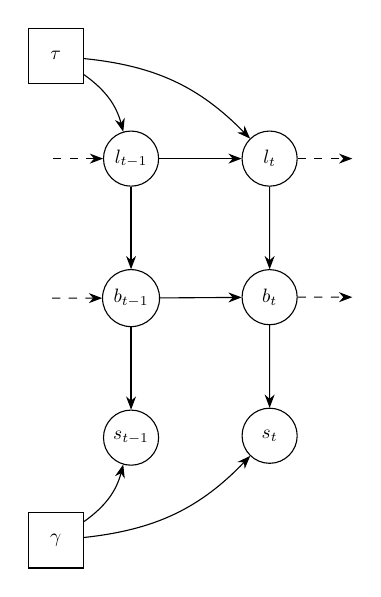
\begin{tikzpicture}[
    scale=0.7, % Adjust this value (e.g., 0.7, 0.9) as needed
    transform shape, % Ensures node text scales with the node
    node distance=1.5cm and 1.5cm, % Original distances
    latent/.style={circle, draw, minimum size=1cm},
    param/.style={rectangle, draw, minimum size=1cm},
    >=Stealth]

  % Place nodes for time t-1
  \node (ltm1) [latent] {$l_{t-1}$};
  \node (btm1) [latent, below=of ltm1] {$b_{t-1}$};
  \node (stm1) [latent, below=of btm1] {$s_{t-1}$};

  % Place nodes for time t
  \node (lt) [latent, right=of ltm1] {$l_t$};
  \node (bt) [latent, below=of lt] {$b_t$};
  \node (st) [latent, below=of bt] {$s_t$};

  % Place parameter nodes
  \node (tau) [param, above left=1cm and 0.5cm of ltm1] {$\tau$};
  \node (gamma) [param, below left=1cm and 0.5cm of stm1] {$\gamma$};

  % Draw edges (arrows)
  \draw [->] (tau) edge [bend left=20] (ltm1);
  \draw [->] (tau) edge [bend left=20] (lt);
  \draw [->] (ltm1) -- (lt);
  \draw [->] (ltm1) -- (btm1); % As shown in the diagram
  \draw [->] (lt) -- (bt);
  \draw [->] (btm1) -- (bt);
  \draw [->] (btm1) -- (stm1); % As shown in the diagram
  \draw [->] (bt) -- (st);   % Standard HMM dependency

  % Edges from gamma (as shown in diagram)
  \draw [->] (gamma) edge [bend right=20] (stm1);
  \draw [->] (gamma) edge [bend right=20] (st);

  % Draw dashed lines indicating time sequence
  \draw [dashed, <-] (ltm1) -- ++(-1.5, 0); % From l_{t-1} leftwards
  \draw [dashed, ->] (lt) -- ++(1.5, 0);   % From l_t rightwards
  \draw [dashed, <-] (btm1) -- ++(-1.5, 0); % From b_{t-1} leftwards
  \draw [dashed, ->] (bt) -- ++(1.5, 0);   % From b_t rightwards
  \end{tikzpicture}
  \end{center}
\end{frame}

\begin{frame}
  \frametitle{Hidden Markov Model forward pass}
  \begin{center}
    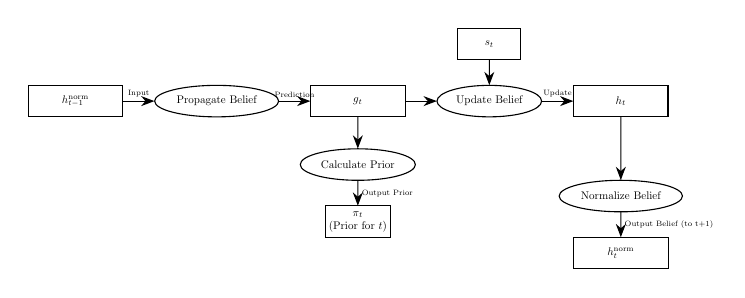
\begin{tikzpicture}[
    scale=0.4, transform shape, % Keep scaling
    node distance=1cm and 1cm, % Adjust vertical/horizontal distance
    % --- MINIMALIST STYLES ---
    base_node/.style={draw, minimum width=2.5cm, minimum height=1cm, align=center, fill=white},
    latent/.style={circle, draw, minimum size=1cm},
    belief/.style={base_node, minimum width=3cm},
    process/.style={base_node, ellipse},
    io/.style={base_node, minimum width=2cm},
    >=Stealth
]

% --- ROW 1 ---
\node (h_prev) [belief] {$h_{t-1}^{\text{norm}}$};
\node (propagate) [process, right=of h_prev] {Propagate Belief};
\node (g_t) [belief, right=of propagate] {$g_t$};
\node (update) [process, right=of g_t] {Update Belief};
\node (s_t) [io, above=0.8cm of update] {$s_t$}; % Input Stimulus
\node (h_t_unnorm) [belief, right=of update] {$h_t$};

% --- ROW 2 (Prior Calculation Branch) ---
\node (calc_prior) [process, below=1cm of g_t] {Calculate Prior}; % Below g_t
\node (pi_t) [io, below=0.8cm of calc_prior] {$\pi_t$ \\ (Prior for $t$)}; % Below calc_prior

% --- ROW 3 (Normalization Branch - WRAPPED) ---
\node (normalize) [process, below=2cm of h_t_unnorm] {Normalize Belief}; % Position below the end of row 1
\node (h_t_norm) [belief, below=0.8cm of normalize] {$h_{t}^{\text{norm}}$}; % Final output

% Edges (Arrows) - Adjusted for wrapped layout
\draw [->] (h_prev) -- (propagate) node[midway, above, font=\scriptsize] {Input};
\draw [->] (propagate) -- (g_t) node[midway, above, font=\scriptsize] {Prediction};
\draw [->] (g_t) -- (calc_prior);
\draw [->] (calc_prior) -- (pi_t) node[midway, right, font=\scriptsize] {Output Prior};
\draw [->] (g_t) -- (update);
\draw [->] (s_t) -- (update); % Removed label for space
\draw [->] (update) -- (h_t_unnorm) node[midway, above, font=\scriptsize] {Update};
\draw [->] (h_t_unnorm) -- (normalize);
\draw [->] (normalize) -- (h_t_norm) node[midway, right, font=\scriptsize] {Output Belief (to t+1)};


\end{tikzpicture}
  \begin{itemize}
      \tiny
    \item Propagate belief: \begin{equation}\label{eq:1}
        g_{t}(l_{t}, b_{t}) = \sum_{l_{t-1}, b_{t-1}} h_{t-1}(l_{t-1}, b_{t-1}) \cdot P(l_{t} | l_{t-1}) \cdot P(b_{t} | b_{t-1}, l_{t})
    \end{equation}
    \item Calculate prior: \begin{equation}\label{eq:2}
        \pi_{t} = 0.5 \cdot P(b_{t}=0|s_{1:(t-1)}) + \gamma \cdot P(b_{t}=1|s_{1:(t-1)}) + (1-\gamma) \cdot P(b_{t}=-1|s_{1:(t-1)})
    \end{equation}
      \begin{equation}\label{eq:3}
        P(b_{t}=k | s_{1:(t-1)}) = \frac{\sum_{l_{t}} g_{t}(l_{t}, b_{t}=k)}{\sum_{l_{t}, b_{t}} g_{t}(l_{t}, b_{t})}
    \end{equation}
  \item Update belief: \begin{equation}\label{eq:4}
      h_{t}(l_{t}, b_{t}) = P(s_{t}|b_{t}) \cdot g_{t}(l_{t}, b_{t})
  \end{equation}
  \end{itemize}
  \end{center}
\end{frame}

\begin{frame}
  \frametitle{Task mechanics and Bayesian prior predictions}
  \begin{center}
    \includegraphics[width=0.5\textwidth, keepaspectratio]{./figure1b}
  \end{center}
  \begin{itemize}
    \item $P(s_{t} = 1) = 0.2 or 0.8$
    \item For 90 trials $s_{t} = 0$
    \item Block length $H_{\tau}(n), n \geq 20, n \leq 100, \tau = 60$
    \item Positive feedback = water, Negative feedback = white noise + timeout
    \item Next trial after delay + wheel fixed
  \end{itemize}
\end{frame}

\begin{frame}
  \frametitle{Prior-based mechanism $>$ action bias}
  \begin{center}
    \includegraphics[width=0.5\textwidth, keepaspectratio]{./figure1c}
  \end{center}
  \begin{itemize}
    \item Negative values = stimulus on left
    \item Positive values = stimulus on right
    \item Zero = no contrast stimulus
  \end{itemize}
\end{frame}

\begin{frame}
  \frametitle{Performance recovers slower than predicted by agent sampling prior}
  \begin{center}
    \includegraphics[width=0.5\textwidth, keepaspectratio]{./figure1d}
  \end{center}
  \begin{itemize}
    \item $p(\text{correct at trial } t) =
\begin{cases}
B + (A-B) \cdot e^{-t/\tau} & \text{if } t \ge 0 \\
B & \text{if } t < 0
\end{cases}$
  \item A and B are free parameters, A = performance drop, B = asymptotic performance
  \end{itemize}
\end{frame}

\begin{frame}
  \frametitle{Prior decoding during the ITI}
  \begin{center}
    \includegraphics[width=0.65\textwidth, keepaspectratio]{./figure2a}
  \end{center}
  \begin{itemize}
      \small
    \item Single cell recording (almost, spike-sorting) using neuropixels
    \item Decoding is a LASSO linear regression $\hat{y_{i}} = x_{i}w+b$ over Bayes-optimal prior $\pi_{t}$
    \item LASSO shrinks uncorrelated neuron activity, and is robust to outlier (drift)
    \item $ORB_{vl}$ value representation, cross validation reporting median $R^{2}$
  \end{itemize}
\end{frame}

\begin{frame}
  \frametitle{Prior decoding during the ITI}
  \begin{center}
    \includegraphics[width=0.35\textwidth, keepaspectratio]{./figure2b}
  \end{center}
  \begin{itemize}
    \item Wide Field Calcium Imaging, aggregate cortical activity
    \item $VGCCs \rightarrow Calcium \ influx \rightarrow Vesicle \ fusion \rightarrow GECI \rightarrow Bright$
    \item Merge maps with Fisher's combined probability test
    \item Sensory, Associative, Motor, Sub-cortical
  \end{itemize}
\end{frame}

\begin{frame}
  \frametitle{Prior decoding during the ITI}
  \begin{center}
    \includegraphics[width=0.65\textwidth, keepaspectratio]{./figure2c}
  \end{center}
  \begin{itemize}
    \item Cross-modal comparison
  \end{itemize}
\end{frame}

\begin{frame}
  \frametitle{Both modalities are correlated in decoding}
  \begin{center}
    \includegraphics[width=0.65\textwidth, keepaspectratio]{./figure2d}
  \end{center}
  \begin{itemize}
    \item Cross-modal comparison
  \end{itemize}
\end{frame}

\begin{frame}
  \frametitle{Decoded signal strength coincides with theoretical importance of prior}
  \begin{center}
    \includegraphics[width=0.65\textwidth, keepaspectratio]{./figure2e}
  \end{center}
  \begin{itemize}
    \item Zero-contrast trials represent prior-guided action (psychometric curves)
    \item $P(s_{t} = Right | History, Evidence \rightarrow 0) = \pi_{t}$
  \end{itemize}
\end{frame}

\begin{frame}
  \frametitle{Neuron prior model $>$ Embodied model}
  \begin{center}
    \includegraphics[width=0.5\textwidth, keepaspectratio]{./figure2f}
  \end{center}
  \begin{itemize}
    \item Better region prior decoding predicts increased $residuals_{Bayes \ prior - Embodied \ features}$
    \item Prior decoding regions decode Emobodied residuals
    \item $Residuals_{Embodied \ model} = \beta_{0} + \beta_{Neuron \ activity}$
  \end{itemize}
\end{frame}

\begin{frame}
  \frametitle{Evidence for the 'Bayesian network'}
  \begin{center}
    \includegraphics[width=0.7\textwidth, keepaspectratio]{./figure2g}
  \end{center}
  \begin{itemize}
    \item Brain-wide bi-directional network encode prior
    \item Non-hierarchical modulation of sensory areas
  \end{itemize}
\end{frame}

\begin{frame}
  \frametitle{Evidence for the 'Bayesian network'}
  \begin{center}
    \includegraphics[width=0.3\textwidth, keepaspectratio]{./figure2h}
  \end{center}
  \begin{itemize}
    \item Pseudosession: $Sample \ from \ G_{mechanism} \rightarrow build \ M \ series \rightarrow compute \ \pi_{synthetic} \rightarrow GC(\pi_{synthetic})$
  \end{itemize}
\end{frame}

\begin{frame}
  \frametitle{Neurometric curves}
  \begin{center}
    \includegraphics[width=0.5\textwidth, keepaspectratio]{./figure3a}
  \end{center}
  \begin{itemize}
    \item Post-stimulus measurement
    \item Determine if the prior persists and biases the integration of stimulus
    \item Action is greedy over decoded prior, represent 'update belief'
  \end{itemize}
\end{frame}

\begin{frame}
  \frametitle{Neurometric curves}
  \begin{center}
    \includegraphics[width=0.5\textwidth, keepaspectratio]{./figure3b}
  \end{center}
  \begin{itemize}
    \item Same but for ITI data
    \item Separation is significant but significantly reduced
    \item This is just the prior
  \end{itemize}
\end{frame}

\begin{frame}
  \frametitle{Neurometric curves}
  \begin{center}
    \includegraphics[width=0.5\textwidth, keepaspectratio]{./figure3c}
  \end{center}
  \begin{itemize}
    \item The shift is similar for cell-level and aggregate data
  \end{itemize}
\end{frame}

\begin{frame}
  \frametitle{Neurometric curves}
  \begin{center}
    \includegraphics[width=0.8\textwidth, keepaspectratio]{./figure3d}
  \end{center}
  \begin{itemize}
    \item Areas that strongly decode the prior, also show higher level of bias post stimulus
  \end{itemize}
\end{frame}

\begin{frame}
  \frametitle{Neurometric curves}
  \begin{center}
    \includegraphics[width=0.5\textwidth, keepaspectratio]{./figure3e}
  \end{center}
  \begin{itemize}
    \item From belief propagation to 'update belief' the prior is represented brain-wide
  \end{itemize}
\end{frame}

\begin{frame}
  \frametitle{Heuristic models comparison}
  \begin{center}
    \includegraphics[width=0.3\textwidth, keepaspectratio]{./figure4a}
  \end{center}
  \begin{itemize}
    \item Model selection favored the action kernel heuristic
      \begin{equation}
        \pi_{t} = (1 - \alpha) \pi_{t-1} + \alpha \cdot [s_{t-1} = Right]
      \end{equation}
      \begin{equation}
        \pi_{t} = (1 - \alpha) \pi_{t-1} + \alpha \cdot [a_{t-1} = Right]
      \end{equation}
  \end{itemize}
\end{frame}

\begin{frame}
  \frametitle{Heuristic models comparison}
  \begin{center}
    \includegraphics[width=0.5\textwidth, keepaspectratio]{./figure4b}
  \end{center}
  \begin{itemize}
    \item Action kernel heuristic is near optimal
    \item $\tau_{optimal} \approx \tau_{empirical}$
  \end{itemize}
\end{frame}

\begin{frame}
  \frametitle{Heuristic models comparison}
  \begin{center}
    \includegraphics[width=0.55\textwidth, keepaspectratio]{./figure4c}
  \end{center}
  \begin{itemize}
    \item Action kernel better captures effects of being wrong at $t-1$
    \item This is consistent with neural prior
  \end{itemize}
\end{frame}

\begin{frame}
  \frametitle{Heuristic models comparison}
  \begin{center}
    \includegraphics[width=0.55\textwidth, keepaspectratio]{./figure4d}
  \end{center}
  \begin{itemize}
    \item Decoding the action kernel provides better fit with neural activity
  \end{itemize}
\end{frame}

\begin{frame}
  \frametitle{Moving average models evidence}
  \begin{center}
    \includegraphics[width=0.7\textwidth, keepaspectratio]{./figure4e}
  \end{center}
  \begin{itemize}
    \item Neural prior considers past ~5 trials of information
    \item Normalized coefficients
    \item Stepwise regression
  \end{itemize}
\end{frame}

\begin{frame}
  \frametitle{Moving average models evidence}
  \begin{center}
    \includegraphics[width=0.8\textwidth, keepaspectratio]{./figure4f}
  \end{center}
  \begin{itemize}
    \item 'Memory' is present in behavioral and neural fits
    \item Action kernel strategy is likely implemented by neural activity
  \end{itemize}
\end{frame}

\begin{frame}
  \frametitle{Conclusion}
  \begin{center}
    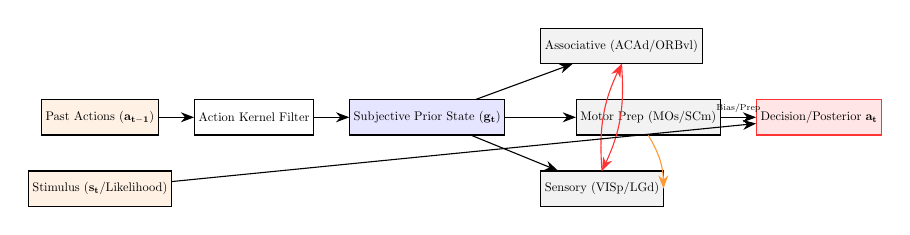
\begin{tikzpicture}[
    scale=0.45, transform shape,
    node distance=1cm and 1cm, % Standard separation
    % --- MINIMALIST STYLES ---
    module/.style={rectangle, draw, minimum width=3cm, minimum height=1cm, fill=white, align=center},
    hub/.style={module, draw, fill=blue!10, minimum width=4cm}, % Central Prior State
    region/.style={module, minimum width=2.5cm, fill=gray!10}, % Specific Brain Region
    io/.style={module, fill=orange!10, minimum width=2cm}, % Input/Output
    >=Stealth
]

% --- 1. PRIOR GENERATION (Input) ---
\node (act_hist) [io] {Past Actions ($\mathbf{a_{t-1}}$)};
\node (filter) [module, right=of act_hist] {Action Kernel Filter};

% --- 2. CENTRAL STATE (HUB) ---
% This node represents the Subjective Prior (log g_t)
\node (prior_state) [hub, right=of filter, node distance=2.5cm] {Subjective Prior State ($\mathbf{g_t}$)};

% --- 3. WIDESPREAD ENCODING NETWORK ---
\node (assoc) [region, above right=of prior_state] {Associative (ACAd/ORBvl)};
\node (sensory) [region, below right=of prior_state] {Sensory (VISp/LGd)};
\node (motor) [region, right=2cm of prior_state] {Motor Prep (MOs/SCm)};


% --- 4. DECISION AND CLOSURE ---
\node (stim) [io, below=of act_hist] {Stimulus ($\mathbf{s_t}$/Likelihood)};
\node (posterior) [io, right=1cm of motor, fill=red!10, draw=red!80] {Decision/Posterior $\mathbf{a_t}$};


% --- FLOWS ---

% 1. Prior Generation (Input)
\draw [->] (act_hist) -- (filter);
\draw [->] (filter) -- (prior_state);

% 2. Network Encoding (All regions encode the central state)
\draw [->] (prior_state) -- (assoc);
\draw [->] (prior_state) -- (sensory);
\draw [->] (prior_state) -- (motor);

% 3. Recurrent Loops (Core Findings 2G/2H)
% Assoc <-> Sensory Loop
\draw [->,color=red!80] (assoc.south) to [bend left=15] (sensory.north) node[midway, left, font=\scriptsize] {};
\draw [->,color=red!80] (sensory.north) to [bend left=15] (assoc.south) node[midway, right, font=\scriptsize] {};

% Associative/Motor to Sensory Feedback (Against traditional hierarchy)
\draw [->, color=orange!80, bend left=15] (motor.south) to (sensory.east);

% 4. Decision Integration
\draw [->] (stim) -- (posterior);
\draw [->] (motor) -- (posterior) node[midway, above, font=\scriptsize] {Bias/Prep};

% 5. Behavioral Loop Closure

\end{tikzpicture}
  \end{center}
\end{frame}

\end{document}
